%%%%%%%%%
\section{Graded unitarity constraints on $V_k(\mathfrak{e}_{n=6,7,8})$} \label{sec:typeEgrunit}
%%%%%%%%%
In this section, we complete our characterisation by studying graded unitarity constraints on simply-laced exceptional affine Kac--Moody algebras. The approach will be similar to that used in Sections \ref{sec:typeAgrunit} and \ref{sec:typeDgrunit}. We will first perform a low-level graded unitarity analysis, assemble a variety of data about the representations (and their root multiplicities) of the primitive null states corresponding to a specific set of zeros of the vacuum determinant, and then impose all-level determinant-based graded unitarity sign constraints from \eqref{eq:grunitsignrule}, leading to constraints on the level $k$.\footnote{All calculations in this section were performed using \texttt{SageMath}. For all relevant cases, the primitive null representations first appeared in \cite{jiang2025singular}, while for many cases, the relevant root multiplicities can be found in \cite{Lübeck_2001}.} While we investigate the $V_k(\mathfrak{e}_6)$ case in necessary detail, we keep the discussion of the $V_k(\mathfrak{e}_7)$ and $V_k(\mathfrak{e}_8)$ affine VOAs brief and mention only the relevant results of various computations.

%%%%%%%%%
\subsection{$V_k(\mathfrak{e}_6)$}
%%%%%%%%%
%------------------------------------------------
% E_6
%------------------------------------------------
\begin{figure} 
\centering
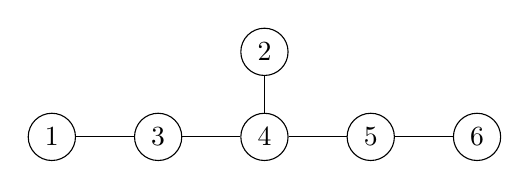
\begin{tikzpicture}[scale=0.9,
    every node/.style={circle, draw, fill=white, inner sep=2pt, minimum size=6mm}]
    
    % Nodes
    \node (1) at (0,0)   {$1$};
    \node (2) at (1.5,0) {$3$};
    \node (3) at (3,0)   {$4$};
    \node (4) at (4.5,0) {$5$};
    \node (5) at (6,0) {$6$};
    \node (6) at (3,1.2) {$2$};

    % Edges
    \draw (1)--(2)--(3)--(4)--(5);
    \draw (3)--(6);

\end{tikzpicture}
\caption{Dynkin diagram of $E_6$} \label{fig:E6Dynkindiagram}
\end{figure} 
%%%%%%%%%
For the $V_k(\mathfrak{e}_6)$ affine VOA, we follow the usual convention in which the Dynkin diagram of $E_6$ is given by Figure \ref{fig:E6Dynkindiagram}. Before investigating graded unitarity constraints, as with the analyses in the previous sections, we first note that the constraints on $A_{(t,\alpha)}$ that are consistent with the regularity criterion \eqref{eq:ADEregularity} are given by,
\begin{equation} \label{eq:Atconste6}
    A_{(t,\alpha)} \ \ \begin{cases}
        = 12 \qquad \text{when} \ \ t = 1 \ \ \text{and} \ \ \alpha = \theta \\ = 12 \qquad \text{when} \ \ t = 2 \ \ \text{and} \ \ \alpha = (0,1,1,1,1,0) =: \alpha^{\mathfrak{e}_6}_{(2)} \\ = 12 \qquad \text{when} \ \ t = 3 \ \ \text{and} \ \ \alpha = (0,0,0,1,0,0) =: \alpha^{\mathfrak{e}_6}_{(3)} \\ \geqslant 18 \qquad \text{otherwise}
    \end{cases}
\end{equation}
Moreover, note that while $2\alpha^{\mathfrak{e}_6}_{(2)}$ and $3\alpha^{\mathfrak{e}_6}_{(3)}$ are not regular dominant, their regular dominant representatives in the Weyl orbit can be found using a series of Weyl reflections to be the highest root. As a result, one obtains that, 
\begin{equation}
    \frac{E(\theta)}{E(0)} = -\frac{E(2\alpha^{\mathfrak{e}_6}_{(2)})}{E(0)} = -\frac{E(3\alpha^{\mathfrak{e}_6}_{(3)})}{E(0)} = \text{ch Ad}~.
\end{equation}
%%%%%%%%%%%
\subsubsection{Bespoke low-level analysis}
In this case, it is useful to perform a low-level analysis up to $L = 4$. To this end, the fixed-root vacuum determinant for conformal levels $L \leqslant 4$ takes the following form, 
\begin{equation} \label{eq:lowlevele6det1to4}
\begin{split}
    &\text{det}~S_{\delta + \alpha} \qquad \propto \textcolor{blue}{(k - 0)}~, \\
    &\text{det}~S_{2\delta + \alpha} \ \ \ \ \ \propto \textcolor{blue}{(k + 3)^5}(k - 0)^{\#_1} (\ldots \ldots)~, \\ 
    &\text{det}~S_{3\delta + \omega_1 + \omega_6} \propto \textcolor{blue}{(k + 6)(k + 4)^4} (k + 3 )^{\#} (\ldots \ldots)~, \\
    &\text{det}~S_{4\delta + \alpha} \ \ \ \ \ \propto \textcolor{blue}{(k + 9)^{1}(k + 15/2)^5}(k+6)^{\#} (\ldots \ldots)~. \\
\end{split}
\end{equation}
Up to $L  = 2$, determinant based graded unitarity constraints lead to $-12 < k \leqslant -3$ or $k = 0$. At $L = 3$, the null states at $k = -6$ and $k = -4$ are components of the $V_{\omega_1+\omega_6}$ and $V_{\omega_4}$ representations respectively. While determinant-based constraints already rule out $k \in (-6,-4) \bigcup (-4,-3)$, since the null states at $k = -6$ and $k = -4$ are components of different representations, passing to a representation basis further rules out $k = -4$. This leads to the constraints $-12 < k \leqslant -6$ or $k = \{-3,0\}$. At $L = 4$, the null states corresponding to the zeros at $k = -9$ and $k = -15/2$ are components of the adjoint and $V_{\omega_1+\omega_6}$ representation respectively, and a similar analysis as at $L = 3$ rules out $k \in (-9,-6)$. This leads to the following graded unitarity constraints up to $L \leqslant 4$,
\begin{equation} \label{eq:e6lowlevelconst}
    -12<k \leqslant -9 \qquad \text{or} \qquad k = \left\{-6, -3, 0 \right\}~.
\end{equation}
We now turn to investigating the structure of zeros for $L \geqslant 6$, and implementing all-level determinant-based graded unitarity constraints on $V_k(\mathfrak{e}_6)$.
%%%%%%%%%%%%%%%%%%%%%%%%%%%
\begin{table}[] 
    \centering
    \begin{tabular}{|c|c|c|c|}
        \hline\hline
        $k$ & $L_s$ & Representation & Multiplicity \\
        \hline\hline
        $k_{2,q}$  & $12q$ & $V_{\omega_4} = \textbf{2925}$ & $15$ \\
        $k_{3,q}$  & $4q$  & $V_\theta = \textbf{78}$ & $1$ \\
        $k_{4,q}$  & $12q$ & $V_{\omega_1+2\omega_2 + \omega_6} = \textbf{812175}$ & $1085$ \\
        $k_{6,q}$  & $3q$  & $V_{\omega_1 + \omega_6} = \textbf{650}$ & $5$ \\
        $k_{12,q}$ & $q$   & $V_\theta = \textbf{78}$ & $1$ \\
        \hline
    \end{tabular}
    \caption{\label{tb:e6zerodata} Smallest conformal level $L_s$, primitive null representations and their root multiplicities for different values of $k$.}
\end{table}
%%%%%%%%%%%%%%%%%%%%%%%%%%%
%%%%%%%%%%%%
\subsubsection{Structure of zeros and all-level graded unitarity constraints}
%%%%%%%%%%%%
We first assemble data relevant for understanding the structure of zeros of the fixed-root vacuum determinant. In particular, Table \ref{tb:e6zerodata} collects the smallest conformal level $L_s$ at which $k = k_{2,q}, k_{3,q}, k_{4,q}, k_{6,q}$, and $k_{12,q}$ first appear as zeros of the fixed-root vacuum determinant. In addition, we also note the representation of the primitive null state at these zeros, and the root multiplicity of the representation. 

To provide a glimpse into the computation of the representation and root multiplicity appearing in Table \ref{tb:e6zerodata}, note that a direct computation using \eqref{eq:expinchar} and \eqref{eq:Atconste6} implies,
\begin{equation} \label{eq:multrelevante6}
\begin{split}
    &\frac{M_{12/q,q}}{E(0)} = \frac{E(\theta)}{E(0)} = \text{ch}~\text{Ad} \qquad \qquad \qquad \qquad \qquad \qquad \text{when} \ \ (12,q) = 1~, \\
    &\frac{M_{3/q,4q}}{E(0)} = \frac{E(\theta)}{E(0)} + \frac{E(2\alpha^{\mathfrak{e}_6}_{(2)})}{E(0)} -\frac{E(3\alpha^{\mathfrak{e}_6}_{(3)})}{E(0)}= \text{ch}~\text{Ad} \qquad \text{when} \ \ (3,q) = 1~.
\end{split}
\end{equation}
As a result, the null states corresponding to the $k = k_{12,q}$ zero (with $(12,q) = 1$) at conformal level $L = q$, and the $k = k_{3,q}$ zero (with $(3,q) = 1$) at conformal level $L = 4q$ both are components of the adjoint representation of $\mathfrak{e}_6$. Consequently, in a fixed-root sector at the respective conformal levels $L$, the multiplicity of these zeros is one.

The relevant data collected in Table \ref{tb:e6zerodata}, together with \eqref{eq:Atconste6} implies that at conformal level $L$, the possible zeros of the fixed-root vacuum determinant are given by,
\begin{equation} \label{eq: e6prelimzero}
    k = \begin{cases}
        k_{12,q} = -12 + \frac{12}{q}: q \leqslant L \ \ \text{and} \ \ (q,12)=1 \\ 
        k_{2,q} = -12 + \frac{2}{q} \ \ : q \leqslant \lfloor \frac{L}{12} \rfloor \ \ \text{and} \ \ (q,2)=1 \\
        k_{3,q} = -12 + \frac{3}{q} \ \ : q \leqslant \lfloor \frac{L}{4} \rfloor \ \ \text{and} \ \ (q,3)=1 \\
        k_{4,q} = -12 + \frac{4}{q} \ \ : q \leqslant \lfloor \frac{L}{12} \rfloor \ \ \text{and} \ \ (q,4)=1 \\
        k_{6,q} = -12 + \frac{6}{q} \ \ : q \leqslant \lfloor \frac{L}{3} \rfloor \ \ \text{and} \ \ (q,6)=1 \\
        k_{A,B} = -12 + \frac{A}{B}: A \geqslant 18 \ \ \text{and} \ \ B \leqslant L
    \end{cases}
\end{equation}


It is convenient to consider the following set of conformal levels $\mathcal{L} = \{1,4,5,7,8,11\}~\text{mod}~12$\footnote{This set comprises all positive integers that are coprime to 12, and positive integers that are multiples of four that are coprime to three.} and split the analysis for conformal levels $L \in \mathcal{L}$ and $L \notin \mathcal{L}$. For a given conformal level $L \in \mathcal{L}$, it can be shown that for $L \geqslant 5$, \footnote{Note that $k = k_{12,L^-}$ is either of the form $k_{12,q}$ with $(12,q) = 1$ or of the form $k_{3,q}$ with $(3,q) = 1$.}
\begin{equation}
    k_{12,L^-} \leqslant k_{18,L}~,
\end{equation}
where $L^-$ denotes the next smallest conformal level in $\mathcal{L}$. As a consequence, \eqref{eq: e6prelimzero} and the multiplicities documented in Table \ref{tb:e6zerodata} lead to the following structure of zeros for the level $L \geqslant 5$ vacuum determinant in a fixed-root sector.
\begin{itemize}
    \item For $L \in \mathcal{L}$, the most negative zero is given by $k = k_{12,L}$ and this zero always appears with multiplicity one. Furthermore, the second most negative zero is given by $k = k_{12,L^-}$. 
    \item For $L \notin \mathcal{L}$, the most negative zero is given by $k = k_{12, L^-}$.
\end{itemize}

The all-level determinant-based graded unitarity constraints now follow almost immediately, given the previously established low-level constraints \eqref{eq:e6lowlevelconst}. First, note that at $L \geqslant 5$ and $L \in \mathcal{L}$, graded unitarity constraints rule out the region $k \in (k_{12, L}, k_{12, L^-})$. On the other hand, at $L \geqslant 5$ and $L \notin \mathcal{L}$, there are no new constraints from graded unitarity. Therefore, one obtains that all-level (fixed root) determinant-based graded unitarity constraints on $V_k(\mathfrak{e}_6)$ rule out all values of the level $k$, except the following.
\begin{equation} \label{eq:e6alllevel}
    k = \begin{cases}
        \textcolor{knownSCFTtext}{k_{12,q} = -12 + \frac{12}{q}: (12,q) = 1} \\
        \textcolor{conjecturedSCFTtext}{k_{3,q} = -12 + \frac{3}{q} \ \ : (3,q) = 1} \\
        \textcolor{knownSCFTtext}{-3} \\ 
        \textcolor{conjecturedSCFTtext}{-6}
    \end{cases}
\end{equation}
The $V_k(\mathfrak{e}_6)$ affine VOAs corresponding to the first set of levels $k = -12+\frac{12}{q}$ with $(12,q) = 1$ are \emph{boundary} admissible, and are precisely the ones associated to ``class-I'' $D_q^{12}(\mathfrak{e}_6)$ Argyres--Douglas SCFTs under the SCFT/VOA correspondence. Moreover, $V_{-3}(\mathfrak{e}_6)$ is precisely the associated VOA of the $E_6$ Minahan-Nemeschansky rank-one SCFT \cite{Minahan:1996fg}.

On the other hand, the affine VOAs corresponding to the levels $k = k_{3,q}$ and $k = -6$ are non-admissible and conjectured to be associated with the $D_{4q}^{12}(\mathfrak{e}_6)$ and $D_{2}^{12}(\mathfrak{e}_6)$ Argyres--Douglas SCFTs respectively. Being non-admissible, it could be that the associated VOAs of these theories are instead non-trivial finite extensions of affine Kac--Moody algebras. Thus, we leave open the possibility that an analogous analysis in a different weight sector or a finer, state-based graded unitarity analysis may rule out some or all of these non-admissible levels. 

%%%%%%%%%
\subsection{$V_k(\mathfrak{e}_7)$}
%%%%%%%%%
%%%%%%%%%
%------------------------------------------------
% E_7
%------------------------------------------------
\begin{figure} \label{fig:E7Dynkindiagram}
\centering
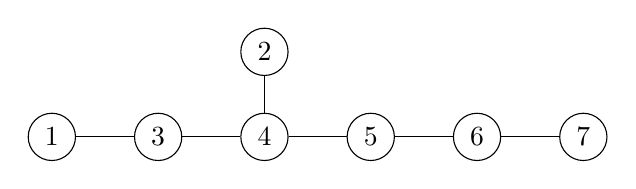
\begin{tikzpicture}[scale=0.9,
    every node/.style={circle, draw, fill=white, inner sep=2pt, minimum size=6mm}]
    
    % Nodes
    \node (1) at (0,0)   {$1$};
    \node (2) at (1.5,0) {$3$};
    \node (3) at (3,0)   {$4$};
    \node (4) at (4.5,0) {$5$};
    \node (5) at (6,0)   {$6$};
    \node (6) at (7.5,0) {$7$};
    \node (7) at (3,1.2) {$2$};

    % Edges
    \draw (1)--(2)--(3)--(4)--(5)--(6);
    \draw (3)--(7);
\end{tikzpicture}
\caption{Dynkin diagram of $E_7$}
\end{figure}
%%%%%%%%%
As with the case of $V_{k}(\mathfrak{e}_6)$, we find the following constraints on $A_{(t,\alpha)}$ that are consistent with the regularity criterion \eqref{eq:ADEregularity},
\begin{equation} \label{eq:Atconste7}
    A_{(t,\alpha)} \ \ \begin{cases}
        = 18 \qquad \text{when} \ \ t = 1 \ \ \text{and} \ \ \alpha = \theta \\ = 18 \qquad \text{when} \ \ t = 2 \ \ \text{and} \ \ \alpha = (1,1,1,2,1,1,0) =: \alpha^{\mathfrak{e}_7}_{(2)} \\ = 18 \qquad \text{when} \ \ t = 3 \ \ \text{and} \ \ \alpha = (0,0,1,1,1,0,0) =: \alpha^{\mathfrak{e}_7}_{(3)} \\ \geqslant 28 \qquad \text{otherwise}
    \end{cases}
\end{equation}
We again emphasise that while $2\alpha^{\mathfrak{e}_7}_{(2)}$ and $3\alpha^{\mathfrak{e}_7}_{(3)}$ are not regular dominant, their regular dominant representative in the Weyl orbit is the highest root. Consequently, one obtains that, 
\begin{equation}
    \frac{E(\theta)}{E(0)} = -\frac{E(2\alpha^{\mathfrak{e}_7}_{(2)})}{E(0)} = -\frac{E(3\alpha^{\mathfrak{e}_7}_{(3)})}{E(0)} = \text{ch Ad}~.
\end{equation}

In this case, the vacuum determinant in an appropriate fixed-weight sector for conformal levels $L \leqslant 5$ is given by, 
\begin{equation} \label{eq:lowlevele7det1to5}
\begin{split}
    &\text{det}~S_{\delta + \alpha} \ \ \ \propto \textcolor{blue}{(k - 0)}~, \\
    &\text{det}~S_{2\delta + \alpha} \ \ \propto \textcolor{blue}{(k + 4)^1}(k - 0)^{\#} (\ldots \ldots)~, \\ 
    &\text{det}~S_{3\delta + 2\omega_7} \propto \textcolor{blue}{(k + 8)} (k + 4 )^{\#} (\ldots \ldots)~, \\
    &\text{det}~S_{4\delta + \omega_6} \ \propto \textcolor{blue}{(k + 11)^{1}(k + 17/2)^4}(k+8)^{\#} (\ldots \ldots)~, \\
     &\text{det}~S_{5\delta + \alpha} \ \ \propto \textcolor{blue}{(k + 72/5)^{1}(k + 12)^5}(k+11)^{\#} (\ldots \ldots)~.
\end{split}
\end{equation}
Up to $L = 3$, determinant based graded unitarity constraints lead to $-18 < k \leqslant -8$ or $k = \{-4,0\}$. At $L = 4$, the null states corresponding to the zeros at $k = -11$ and $k = -17/2$ are components of different representations of $\mathfrak{e}_7$: the $V_{\omega_6}$ and $V_{2\omega_1}$ representation respectively. Thus, passing to a representation basis, graded unitarity rules out the entire region $k \in (-11,-8)$. Similarly, at $L = 5$, the null states corresponding to the zeros at $k = -72/5$ and $k = -12$ are components of the adjoint and $V_{2\omega_7}$ representation, implying that graded unitarity rules out the region $k \in (-72/5, -11)$. To summarise, graded unitarity constraints up to $L \leqslant 5$ restrict the level $k$ to be,
\begin{equation} \label{eq:e7lowlevelconst}
    k \leqslant -\frac{72}{5} \qquad \text{or} \qquad k = \left\{-11, -8, -4, 0 \right\}~.
\end{equation}

%%%%%%%%%%%%%%%%%%%%%%%
\begin{table}[]
    \centering
    \begin{tabular}{|c|c|c|c|}
        \hline\hline
        $k$ & $L_s$ & Representation & Multiplicity \\
        \hline\hline
        $k_{2,q}$  & $9q$ & $V_\theta =\textbf{133}$ & $1$ \\
        $k_{3,q}$  & $14q$  & $V_{\omega_2+\omega_7} = \textbf{40766}$ & $75$ \\
        $k_{6,q}$  & $5q$ & $V_{2\omega_7} = \textbf{1463}$ & $5$ \\
        $k_{9,q}$  & $6q$  & $V_{\omega_4} = \textbf{365750}$ & $390$ \\
        $k_{18,q}$ & $q$   & $V_\theta = \textbf{133}$ & $1$ \\
        \hline
    \end{tabular}
    \caption{\label{tb:e7zerodata} Smallest conformal level $L_s$, primitive null representations and their root multiplicities for different values of $k$.}
\end{table}
%%%%%%%%%%%%%%%%%%%%%%

From the relevant data assembled in Table \ref{tb:e7zerodata} and \eqref{eq:Atconste7}, we find that at conformal level $L$, the possible zeros in a fixed-root vacuum determinant are given by,
\begin{equation} \label{eq: e7prelimzero}
    k = \begin{cases}
        k_{18,q} = -18 + \frac{18}{q}: q \leqslant L \ \ \text{and} \ \ (q,18)=1 \\ 
        k_{2,q} = -18 + \frac{2}{q} \ \ : q \leqslant \lfloor \frac{L}{9} \rfloor \ \ \text{and} \ \ (q,2)=1 \\
        k_{3,q} = -18 + \frac{3}{q} \ \ : q \leqslant \lfloor \frac{L}{14} \rfloor \ \ \text{and} \ \ (q,3)=1 \\
        k_{6,q} = -18 + \frac{6}{q} \ \ : q \leqslant \lfloor \frac{L}{5} \rfloor \ \ \text{and} \ \ (q,6)=1 \\
        k_{9,q} = -18 + \frac{9}{q} \ \ : q \leqslant \lfloor \frac{L}{6} \rfloor \ \ \text{and} \ \ (q,9)=1 \\
        k_{A,B} = -18 + \frac{A}{B}: A \geqslant 28 \ \ \text{and} \ \ B \leqslant L
    \end{cases}
\end{equation}
As with $V_k(\mathfrak{e}_6)$, it is convenient to consider the following set of conformal levels $\mathcal{L} = \{1,5,7,9,11,13,17\}~\text{mod}~18$, and divide the analysis for $L \in \mathcal{L}$ and $L \notin \mathcal{L}$. \footnote{This set comprises all positive integers that are coprime to 18, and positive integers that are \emph{odd} multiples of nine.}  We find that the multiplicities documented in Table \ref{tb:e7zerodata}, and \eqref{eq: e7prelimzero} lead to the following structure of zeros for the level $L \geqslant 6$ vacuum determinant in a fixed-root sector.
\begin{itemize}
    \item For $L \in \mathcal{L}$, the most negative zero is given by $k = k_{18,L}$ and this zero always appears with multiplicity one. Furthermore, the second most negative zero is given by $k = k_{18,L^-}$, where $L^-$ denotes the next smallest conformal level in $\mathcal{L}$. 
    \item For $L \notin \mathcal{L}$, the most negative zero is given by $k = k_{18, L^-}$.
\end{itemize}

Imposing graded unitarity constraints is now almost immediate. First note that determinant-based graded unitarity constraints at $L \geqslant 6$ and $L \in \mathcal{L}$ rule out the region $k \in (k_{18, L}, k_{18, L^-})$. On the other hand, at $L \geqslant 6$ and $L \notin \mathcal{L}$, there are no new constraints from graded unitarity. When combined with the constraints obtained from a bespoke low-level analysis in \eqref{eq:e7lowlevelconst}, one obtains that all-level determinant-based graded unitarity constraints for $V_k(\mathfrak{e}_7)$ rule out all values of $k$, except the following.
\begin{equation} \label{eq:e7alllevel}
    k = \begin{cases}
        \textcolor{knownSCFTtext}{k_{18,q} = -18 + \frac{18}{q}: (18,q) = 1} \\
        \textcolor{conjecturedSCFTtext}{k_{2,q} = -18 + \frac{2}{q} \ \ : (2,q) = 1} \\
        \textcolor{knownSCFTtext}{-4} \\
         -8 \\
          -11
    \end{cases}
\end{equation}
The $V_k(\mathfrak{e}_7)$ affine VOAs with $k$ being the set of boundary-admissible levels above, are precisely the associated VOAs of ``class-I'' $D_q^{18}(\mathfrak{e}_7)$ Argyres--Douglas SCFTs under the SCFT/VOA correspondence. Furthermore, $V_{-4}(\mathfrak{e}_7)$ is the associated VOA of the rank-one $E_7$ Minahan--Nemeschansky SCFT \cite{Minahan:1996cj}. 

The affine VOAs corresponding to the levels $k = k_{2,q}$ are non-admissible and conjectured to be associated with the $D_{9q}^{18}(\mathfrak{e}_7)$. As with the non-admissible cases investigated earlier, it could be that the associated VOAs of these theories are instead non-trivial finite extensions of $V_{k_{2,q}}(\mathfrak{e}_7)$. On the other hand, the affine VOAs corresponding to the remaining levels are not currently known to be associated with any unitary 4d $\mathcal{N} = 2$ SCFTs. In either case, we leave open the possibility that a finer, state-based graded unitarity analysis may rule out some or all of these non-admissible levels. 

%%%%%%%%%
\subsection{$V_k(\mathfrak{e}_8)$}
%%%%%%%%%
In this case, the regularity criterion \eqref{eq:ADEregularity} leads to the following constraints on $A_{(t,\alpha)}$,
\begin{equation} \label{eq:Atconste8}
    A_{(t,\alpha)} \ \ \begin{cases}
        = 30 \qquad \text{when} \ \ t = 1 \ \ \text{and} \ \ \alpha = \theta \\ = 30 \qquad \text{when} \ \ t = 2 \ \ \text{and} \ \ \alpha = (1,1,2,3,2,2,1,1) =: \alpha^{\mathfrak{e}_8}_{(2)} \\ = 30 \qquad \text{when} \ \ t = 3 \ \ \text{and} \ \ \alpha = (0,1,1,2,1,1,1,0) =: \alpha^{\mathfrak{e}_8}_{(3)} \\ = 30 \qquad \text{when} \ \ t = 5 \ \ \text{and} \ \ \alpha = (0,0,0,0,1,0,0,0) =: \alpha^{\mathfrak{e}_8}_{(5)} \\ \geqslant 48 \qquad \text{otherwise}
    \end{cases}
\end{equation}
%%%%%%%%%
%------------------------------------------------
% E_8
%------------------------------------------------
\begin{figure} \label{fig:E8Dynkindiagram}
\centering
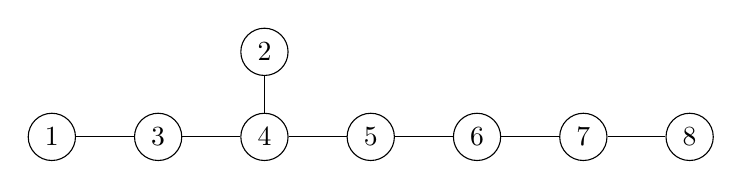
\begin{tikzpicture}[scale=0.9,
    every node/.style={circle, draw, fill=white, inner sep=2pt, minimum size=6mm}]
    
    % Nodes
    \node (1) at (0,0)   {$1$};
    \node (2) at (1.5,0) {$3$};
    \node (3) at (3,0)   {$4$};
    \node (4) at (4.5,0) {$5$};
    \node (5) at (6,0)   {$6$};
    \node (6) at (7.5,0) {$7$};
    \node (7) at (9,0)   {$8$};
    \node (8) at (3,1.2) {$2$};

    % Edges
    \draw (1)--(2)--(3)--(4)--(5)--(6)--(7);
    \draw (3)--(8);
\end{tikzpicture}
\caption{Dynkin diagram of $E_8$}
\end{figure}
%%%%%%%%%

As in the previous cases, the regular dominant weight in the Weyl orbit of $2\alpha^{\mathfrak{e}_8}_{(2)}$ and $3\alpha^{\mathfrak{e}_8}_{(3)}$ is the highest root, leading to, 
\begin{equation}
    \frac{E(\theta)}{E(0)} = -\frac{E(2\alpha^{\mathfrak{e}_8}_{(2)})}{E(0)} = -\frac{E(3\alpha^{\mathfrak{e}_8}_{(3)})}{E(0)} = -\frac{E(5\alpha^{\mathfrak{e}_8}_{(5)})}{E(0)} = \text{ch Ad}~.
\end{equation}

For $V_k(\mathfrak{e}_8)$, note that the vacuum determinant in an appropriate fixed-weight sector for conformal levels $L \leqslant 7$ is given by, 
\begin{equation} \label{eq:lowlevele8det1to7}
\begin{split}
    &\text{det}~S_{\delta + \alpha} \ \ \ \propto \textcolor{blue}{(k - 0)}~, \\
    &\text{det}~S_{2\delta + \omega_1} \ \propto \textcolor{blue}{(k + 6)^1}(k - 0)^{\#} (\ldots \ldots)~, \\ 
    &\text{det}~S_{3\delta + \omega_7} \ \propto \textcolor{blue}{(k + 10)} (k + 6)^{\#} (\ldots \ldots)~, \\
    &\text{det}~S_{4\delta + 2\omega_8} \propto \textcolor{blue}{(k + 29/2)} (k + 10 )^{\#} (\ldots \ldots)~, \\
    &\text{det}~S_{5\delta + \omega_7} \ \propto \textcolor{blue}{(k + 18)} (k + 29/2)^{\#} (\ldots \ldots)~, \\
    &\text{det}~S_{6\delta + \omega_1} \ \propto \textcolor{blue}{(k + 22)^{1}(k + 59/3)^6}(k+18)^{\#} (\ldots \ldots)~, \\
    &\text{det}~S_{7\delta + \alpha} \ \ \propto \textcolor{blue}{(k + 180/7)^1}(k+22)^{\#} (\ldots \ldots)~.
\end{split}
\end{equation}
Determinant-based graded unitarity constraints from \eqref{eq:grunitsignrule} up to $L \leqslant 7$ and passing to a representation basis instead of a weight basis when necessary, we find that compatibility with graded unitarity restricts the level $k$ to be,
\begin{equation} \label{eq:e8lowlevelconst}
    k \leqslant -\frac{180}{7} \qquad \text{or} \qquad k = \left\{-22, -18, -\frac{29}{2}, -10, -6, 0 \right\}~.
\end{equation}

From the relevant data tabulated in Table \ref{tb:e8zerodata} and \eqref{eq:Atconste8}, we find that at conformal level $L$, the possible zeros in a fixed-root vacuum determinant are given by,
\begin{equation} \label{eq: e8prelimzero}
    k = \begin{cases}
        k_{30,q} = -30 + \frac{30}{q}: q \leqslant L \ \ \text{and} \ \ (q,30)=1 \\ 
        k_{2,q} = -30 + \frac{2}{q} \ \ : q \leqslant \lfloor \frac{L}{30} \rfloor \ \ \text{and} \ \ (q,2)=1 \\
        k_{3,q} = -30 + \frac{3}{q} \ \ : q \leqslant \lfloor \frac{L}{31} \rfloor \ \ \text{and} \ \ (q,3)=1 \\
        k_{5,q} = -30 + \frac{5}{q} \ \ : q \leqslant \lfloor \frac{L}{18} \rfloor \ \ \text{and} \ \ (q,5)=1 \\
        k_{6,q} = -30 + \frac{6}{q} \ \ : q \leqslant \lfloor \frac{L}{22} \rfloor \ \ \text{and} \ \ (q,6)=1 \\
        k_{10,q} = -30 + \frac{10}{q} : q \leqslant \lfloor \frac{L}{10} \rfloor \ \ \text{and} \ \ (q,10)=1 \\
        k_{15,q} = -30 + \frac{15}{q} : q \leqslant \lfloor \frac{L}{6} \rfloor \ \ \text{and} \ \ (q,15)=1 \\
        k_{A,B} = -30 + \frac{A}{B} : A \geqslant 48 \ \ \text{and} \ \ B \leqslant L
    \end{cases}
\end{equation}
%%%%%%%%%%%%%%%%%%%%%%%%%
\begin{table}[]
    \centering
    \begin{tabular}{|c|c|c|c|}
        \hline\hline
        $k$ & $L_s$ & Representation & Multiplicity \\
        \hline\hline
        $k_{2,q}$  & $30q$ & $V_{\omega_7} = \textbf{30380}$ & $35$ \\
        $k_{3,q}$  & $31q$  & $V_{\omega_7+\omega_8} = \textbf{4096000}$ & $1624$ \\
        $k_{5,q}$  & $18q$ & $V_{\omega_6} = \textbf{2450240}$ & $1056$ \\
        $k_{6,q}$  & $22q$  & $V_{4\omega_8} = \textbf{79143000}$ & $11705$ \\
        $k_{10,q}$ & $10q$   & $V_{2\omega_1} = \textbf{4881384}$ & $1584$ \\
        $k_{15,q}$ & $6q$   & $V_{\omega_6} = \textbf{2450240}$ & $1056$ \\
        $k_{30,q}$ & $q$   & $V_\theta = \textbf{248}$ & $1$ \\
        \hline
    \end{tabular}
    \caption{\label{tb:e8zerodata} Smallest conformal level $L_s$, primitive null representations and their root multiplicities for different values of $k$.}
\end{table}
%%%%%%%%%%%%%%%%%%%%%%%%

In addition, we note that the multiplicity of the $k = k_{30,q}$ zero in the conformal level $L = q$, fixed-root vacuum determinant is one, as the null state at this zero is a component of the adjoint representation. Motivated by the structure of possible zeros in \eqref{eq: e8prelimzero}, let us define the set $\mathcal{L} = \{1,7,11,13,17,19,23,29\}~\text{mod}~30$, comprising all positive integers coprime to thirty. Along with \eqref{eq: e8prelimzero} and the multiplicities documented in Table \ref{tb:e8zerodata}, this leads to the following structure of zeros for the level $L \geqslant 8$ fixed-root vacuum determinant.
\begin{itemize}
    \item For $L \in \mathcal{L}$, the most negative zero is given by $k = k_{30,L}$ and this zero always appears with multiplicity one. Furthermore, the second most negative zero is given by $k = k_{30,L^-}$. 
    \item For $L \notin \mathcal{L}$, the most negative zero is given by $k = k_{30, L^-}$.
\end{itemize}

The graded unitarity constraints now follow straightforwardly. Determinant-based graded unitarity constraints at $L \geqslant 8$ and $L \in \mathcal{L}$ rule out the region $k \in (k_{30, L}, k_{30, L^-})$. On the other hand, at $L \geqslant 8$ and $L \notin \mathcal{L}$, there are no new constraints. When combined with the results from the bespoke low-level analysis in \eqref{eq:e8lowlevelconst}, one obtains that all-level determinant-based graded unitarity constraints for $V_k(\mathfrak{e}_8)$ rule out all values of $k$, except the following.
\begin{equation} \label{eq:e8alllevel}
    k = \begin{cases}
        \textcolor{knownSCFTtext}{k_{30,q} = -30 + \frac{30}{q}: (30,q) = 1} \\
        \textcolor{knownSCFTtext}{-6} \\
        \textcolor{conjecturedSCFTtext}{-10, -18, -22} \\
        -\frac{29}{2}
    \end{cases}
\end{equation}
The $V_k(\mathfrak{e}_8)$ affine VOAs for  $k$ being the set of boundary-admissible levels above are precisely the associated VOAs of $D_q^{30}(\mathfrak{e}_8)$ ``class I" Argyres--Douglas SCFTs. Furthermore, $V_{-6}(\mathfrak{e}_8)$ is the associated VOA of the rank-one $E_8$ Minahan--Nemeschansky SCFT \cite{Minahan:1996cj}. 

The affine VOAs corresponding to the levels $-10, -18$, and $-22$ are non-admissible, but conjectured to be associated with the $D_{1}^{20}(\mathfrak{e}_8), D_{2}^{24}(\mathfrak{e}_8)$, and $D_{3}^{24}(\mathfrak{e}_8)$ Argyres--Douglas SCFTs respectively. As discussed in Section \ref{sec:intro}, the non-admissibility of these levels does not preclude the associated VOAs of these theories from being non-trivial finite extensions of the corresponding affine Kac--Moody algebras. On the other hand, the affine VOA $V_{-\frac{29}{2}}$, while admissible and quasi-lisse \cite{Arakawa:2010ni, Arakawa:2016hkg}, is not currently known to be associated with any unitary 4d $\mathcal{N} = 2$ SCFTs. Nevertheless, some or all of these levels may be excluded by a more refined state-based analysis of graded unitarity.